\chapter{Rezultati}
\section{Delitev podatkov}
Za končno raziskavo smo izbrali posnetke serij 3, 7 in 11 iz MMID. Vsaka serija vsebuje 109 posnetkov, vsak posnetk 30 primerov stanj, vse skupaj smo jih pridobili 9854. Primere stanj smo skrčili na enakomerno razporeditev, z 2456 primeri vsakega stanja. Sami smo posneli neka minut posnetkov. Vse skupaj 250 primerov stanj, ki smo jih skrčili na enakomerno razporeditev, 62 primerov vsakega stanja. Za učenje nevronskih mrež smo uporabljali množice za učenje z 75\% podatkov in množice za testiranje z 25\% podatkov. Podatki so bili naključno razporejeni med učno in testno množico. Ker smo podatke delili naključno, se lahko posnetki stanj enega prostovoljca pojavijo v učni in testni množici. Pri dodatnem učenju mreže smo uporabili posnetke ene osebe za učenje in testiranje. To skupaj pomeni da sistem ne deluje intersubject. 

\section{Izbira metode povezljivosti}
Ker je kompleksni Pearsonov korelacijski koeficient izračunan iz analitičnih signalov ga lahko definiramo samo za ozke frekvenčne pasove. Pri računanju Grangerjevega indexa vzročnosti te omejitve ni, tako da smo ga lahko računali na celotnem frekvenčnem območju do 45Hz. Prav tako se je pojavilo vprašanje koliko dolgo epoho EEG signala bomo potrebovali za uspešno klasifikacijo. Kot možnosti smo vzeli prvo sekundo, prvi dve sekundi, drugi dve sekundi in prve štiri sekunde po dogodku. Točnost klasifikacije smo ocenili z zgoraj navedeno nevronsko mrežo. Za najboljšo metodo se je izkazal kompleksni Pearsonov korelacijski koeficient na območju 13-30Hz z najdalšimi epohami, 4s.
\begin{figure}[h!]
    \begin{center}
    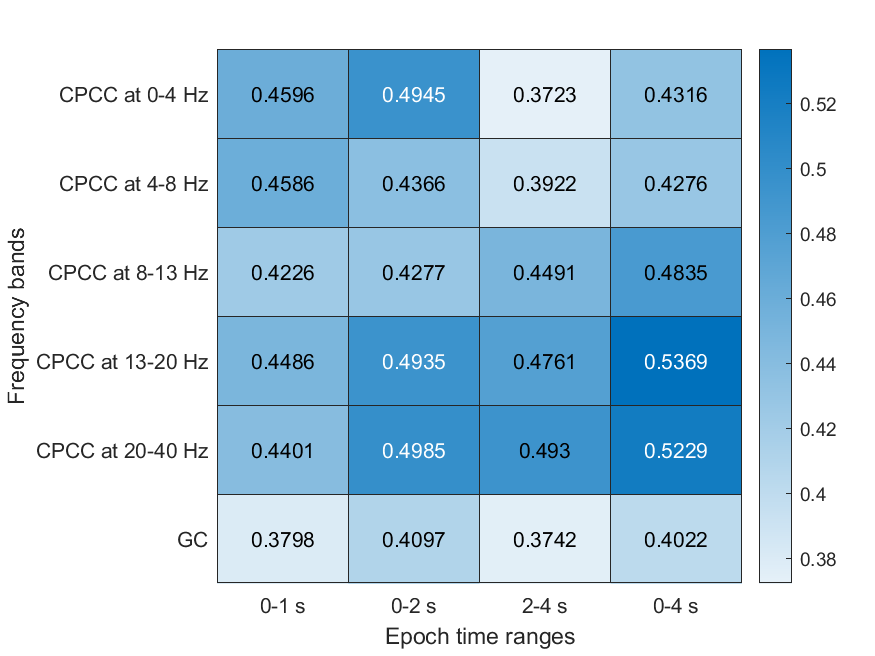
\includegraphics[width=1\linewidth]{slike/Comparison.png}
    \end{center}
    \caption{Primerjava območij in dolžin epoh.}
\end{figure}

\newpage
\subsection{Primerjava filtrov}
Knjižnica EEGLAB vsebuje samo filtre z ničelno fazo, ki filtrirajo naprej in nato nazaj po času, kar v našem primeru ni primerno saj podatke prejemamo sekvenčno, zato smo podatke filtrirali s pomočjo Butterworthovega filtra ki vsebuje stanja. Stanja nam omogočajo filtriranje sekvenčnih podatkov saj preprečijo napako na začetku filtra kjer le ta potrebuje predpostaviti začetno staje vseh signalov 0. Ker filtra nista enakovredna saj prvi ne spreminja faz drugi pa jih zamakne, uporabljena metoda CPCC pa deluje na zamikih faz, smo izvedli dodatno testiranje, da smo preverili če pristop deluje enako učinkovito.
\begin{figure}[h!]
    \begin{center}
    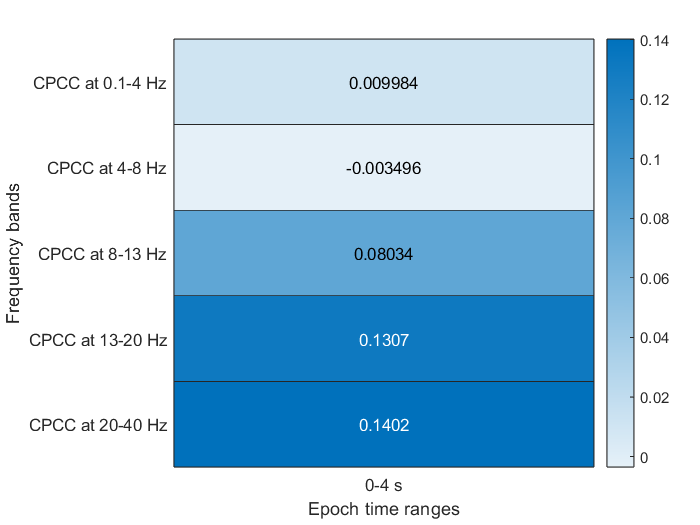
\includegraphics[width=1 \linewidth]{slike/ComparisonFilters.png}
    \end{center}
    \caption{Primerjava klasifikacije CPCC z nevronsko mrežo za epoho 0-4s za različne frekvenčne pasove}
\end{figure}

\begin{figure}[h!]
    \begin{center}
    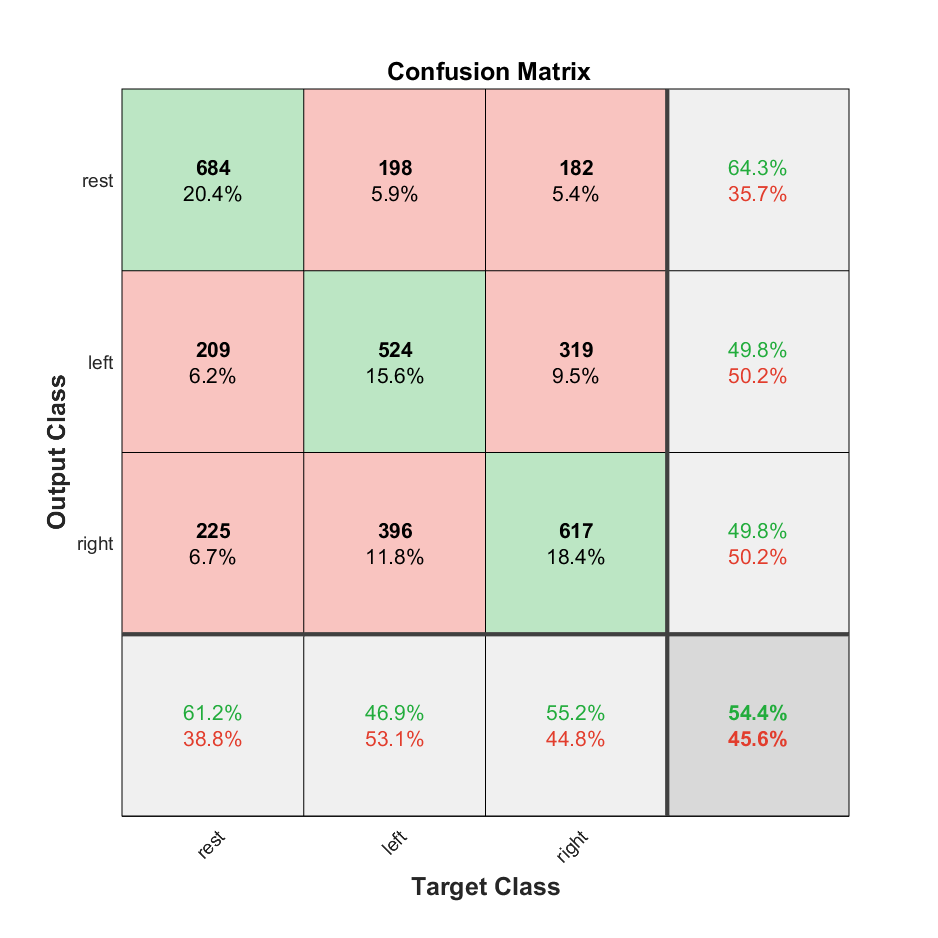
\includegraphics[width=0.5\linewidth]{slike/Confusion_eeglab.png}
    \end{center}
    \caption{Matrika zmede nevronske mreže naučene na podatkih fitriranih s filtrom z ničelno fazo.}
    \end{figure}
    
    \begin{figure}[h!]
    \begin{center}
    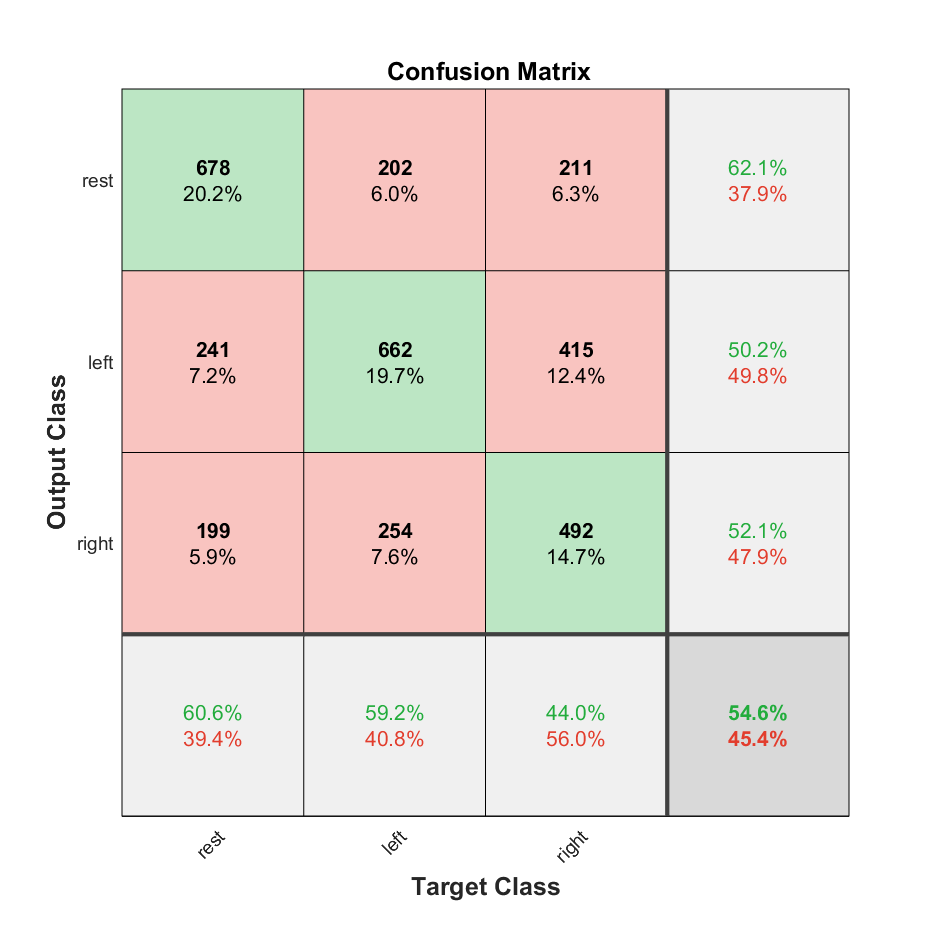
\includegraphics[width=0.5\linewidth]{slike/Confusion_my.png}
    \end{center}
    \caption{Matrika zmede nevronske mreže naučene na podatkih fitriranih z Butterworthovim filtrom.}
    \end{figure}


\newpage
\section{Rezultati na MMID}
\subsection{Classification learner}
Z uporabo aplikacije clasifiacation learner smo testirali več načinov klasifikacije in dosegl 49\% točnost. 
\begin{table}[h]
\centering
\begin{tabular}{|l|l|c|}
\hline
vrsta klasifikacije & metoda & točnost [\%] \\
\hline SVM&Quadratic SVM&53\\
\hline SVM&Linear SVM&53\\
\hline SVM&Medium Gaussian SVM&53\\
\hline Ensemble&Subspace Discriminant&53\\
\hline SVM&Cubic SVM&52\\
\hline Kernel&SVM Kernel&52\\
\hline Kernel&Logistic Regression Kernel&52\\
\hline SVM&Coarse Gaussian SVM&50\\
\hline Efficient Logistic Regression&Efficient Logistic Regression&49\\
\hline Neural Network&Wide Neural Network&49\\
\hline Neural Network&Medium Neural Network&47\\
\hline Efficient Linear SVM&Efficient Linear SVM&46\\
\hline Neural Network&Trilayered Neural Network&45\\
\hline Neural Network&Bilayered Neural Network&45\\
\hline Naive Bayes&Kernel Naive Bayes&45\\
\hline Neural Network&Narrow Neural Network&45\\
\hline Ensemble&Bagged Trees&44\\
\hline KNN&Coarse KNN&44\\
\hline Ensemble&Boosted Trees&43\\
\hline Ensemble&RUSBoosted Trees&42\\
\hline Tree&Medium Tree&41\\
\hline Tree&Fine Tree&41\\
\hline KNN&Cosine KNN&41\\
\hline Tree&Coarse Tree&41\\
\hline KNN&Medium KNN&40\\
\hline KNN&Weighted KNN&40\\
\hline Ensemble&Subspace KNN&40\\
\hline KNN&Cubic KNN&40\\
\hline KNN&Fine KNN&38\\
\hline SVM&Fine Gaussian SVM&37\\

\hline
\end{tabular}
\caption{Točnost klasifikacij}
\end{table}

\subsection{Nevronska mreža}
Nato smo poskusili z nevronsko mrežo ki je dosegla 52\% točnost.

\begin{figure}[h!]
\begin{center}
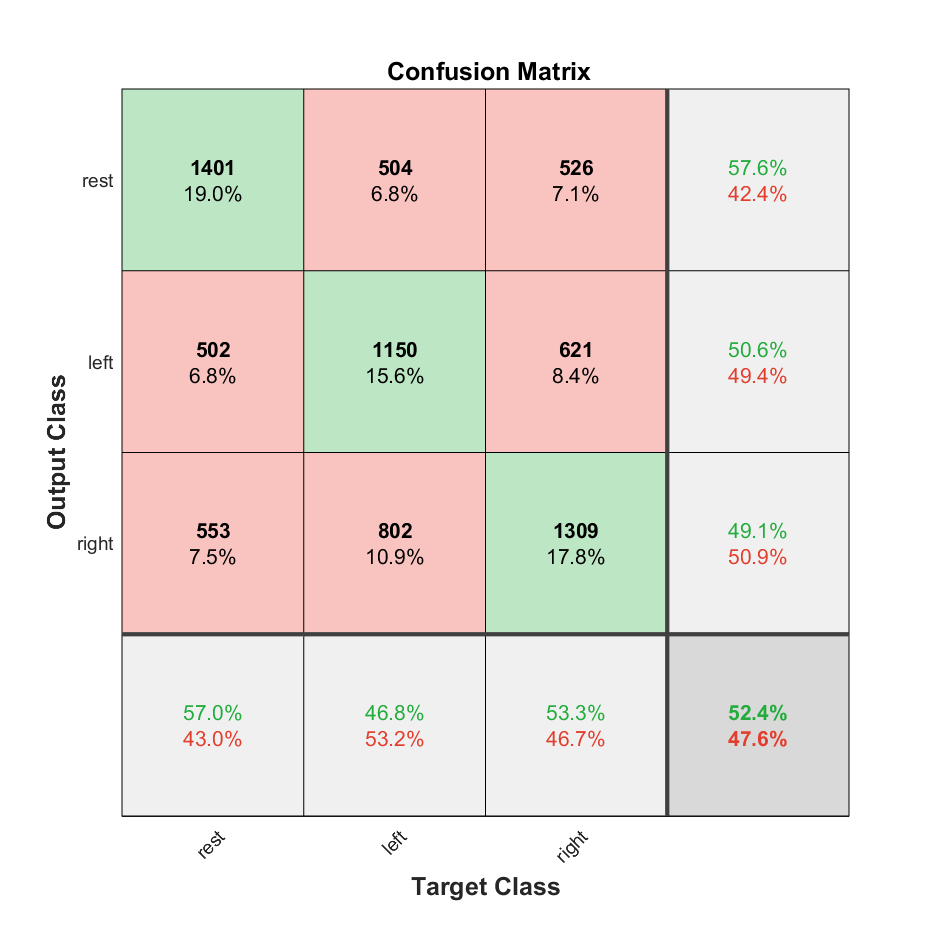
\includegraphics[width=0.5\linewidth]{slike/Confusion_13-20Hz_0s-4s.png}
\end{center}
\caption{Matrika zmede nevronske mreže naučene na podatkih zbirke.}
\end{figure}



\section{Rezultati na lastnih podatkih}
Da bi se približali pogojem v realnem času, smo nevronsko mrežo dodatno naučili na naših podatkih. Zaradi različnih pogojev snemanja in đnčnosti naprav na katerih so podatki snemani je točnost klasifikacije pričakovano padla.
\begin{figure}[h!]
\begin{center}
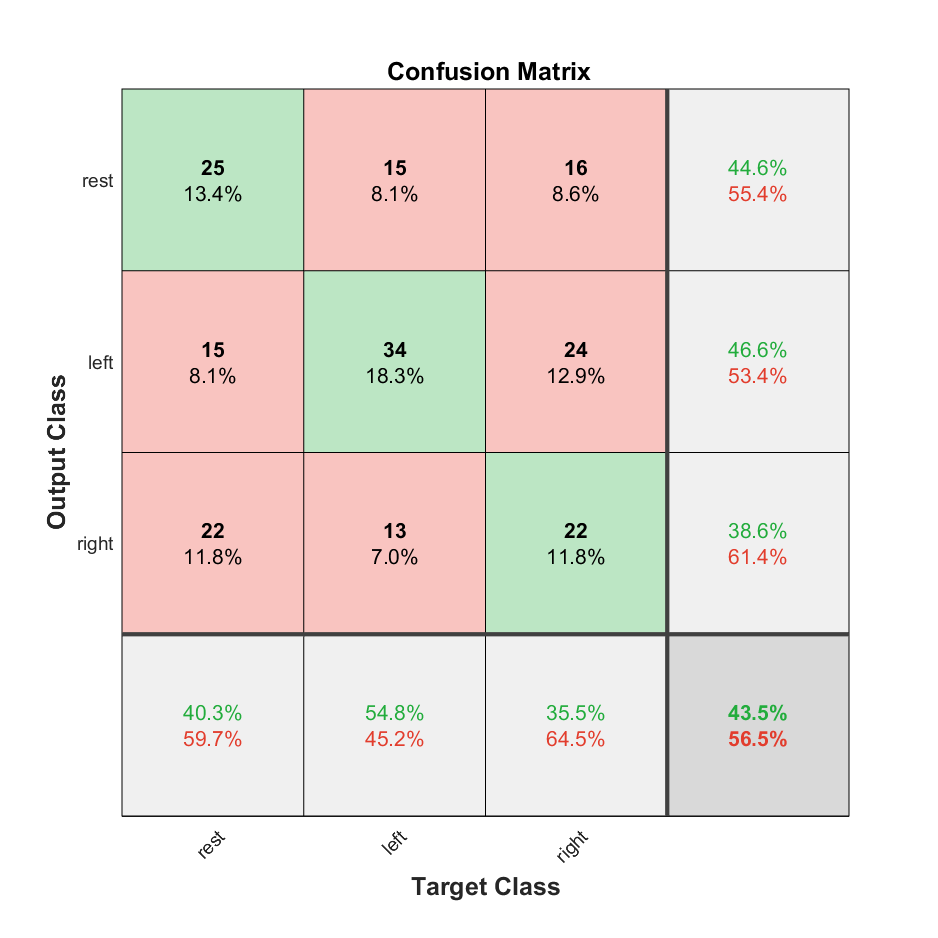
\includegraphics[width=0.5\linewidth]{slike/Confusion_13-20Hz_0s-4s_retrained.png}
\end{center}
\caption{Matrika zmede nevronske mreže dodatno naučene na naših podatkih.}
\end{figure}
\section{Preizkus v realnem času}




